\documentclass{article}

\usepackage{fancyhdr}
\usepackage{ragged2e}
\usepackage{graphicx}
\usepackage{caption}
\usepackage{geometry}
\usepackage{amsmath}
\usepackage{rotating}

\usepackage{listings}
\usepackage{color}

\definecolor{dkgreen}{rgb}{0,0.6,0}
\definecolor{gray}{rgb}{0.5,0.5,0.5}
\definecolor{mauve}{rgb}{0.58,0,0.82}

\lstset{frame=tb,
  language=Java,
  aboveskip=3mm,
  belowskip=3mm,
  showstringspaces=false,
  columns=flexible,
  basicstyle={\small\ttfamily},
  numbers=none,
  numberstyle=\tiny\color{gray},
  keywordstyle=\color{blue},
  commentstyle=\color{dkgreen},
  stringstyle=\color{mauve},
  breaklines=true,
  breakatwhitespace=true,
  tabsize=4
}

% \setcounter{secnumdepth}{1}

% \usepackage{chngcntr}
% \counterwithin{figure}{section}

% \renewcommand*{\thepage}{C\arabic{page}}

% \pagestyle{fancy}
% \lhead{ACME Robotics}
% \chead{\#8367}
% \rhead{\ifcontents Contents \else Week \thesection \fi}

% \newif\ifcontents
% \contentsfalse

\makeatletter
\renewcommand{\@seccntformat}[1]{}
\makeatother

\begin{document}

\subsection{Make a longer and working linear slide for the relic gripper}
%!Reassemble the original slide and make it a single to make it longer and function better.
Ben used the oil to oil the linear slide and noticed that nothing was happening at all. He was helped by Shawn and they found out why the slide wasn't sliding the best. The screws on the sliding plastic piece couldn't be tightened all the way or else the slide wouldn't slide correctly. This happened because the extruded aluminum the slide is made of was being bitten into by the tight screw so it didn't slide smoothly at all. It took a great deal more of force to move the slide than it should have. This was easily solved by un-tightening the screws and making them kind of tight, but not enough to engage the aluminum. This they did and found out the secret of the slide. This took most of the meeting but they still had some time before the end, so they started on the claw to grab the relic. Figure \ref{fig:claw} shows the finished claw gripping the relic.
\begin{figure}[h]
    \centering
    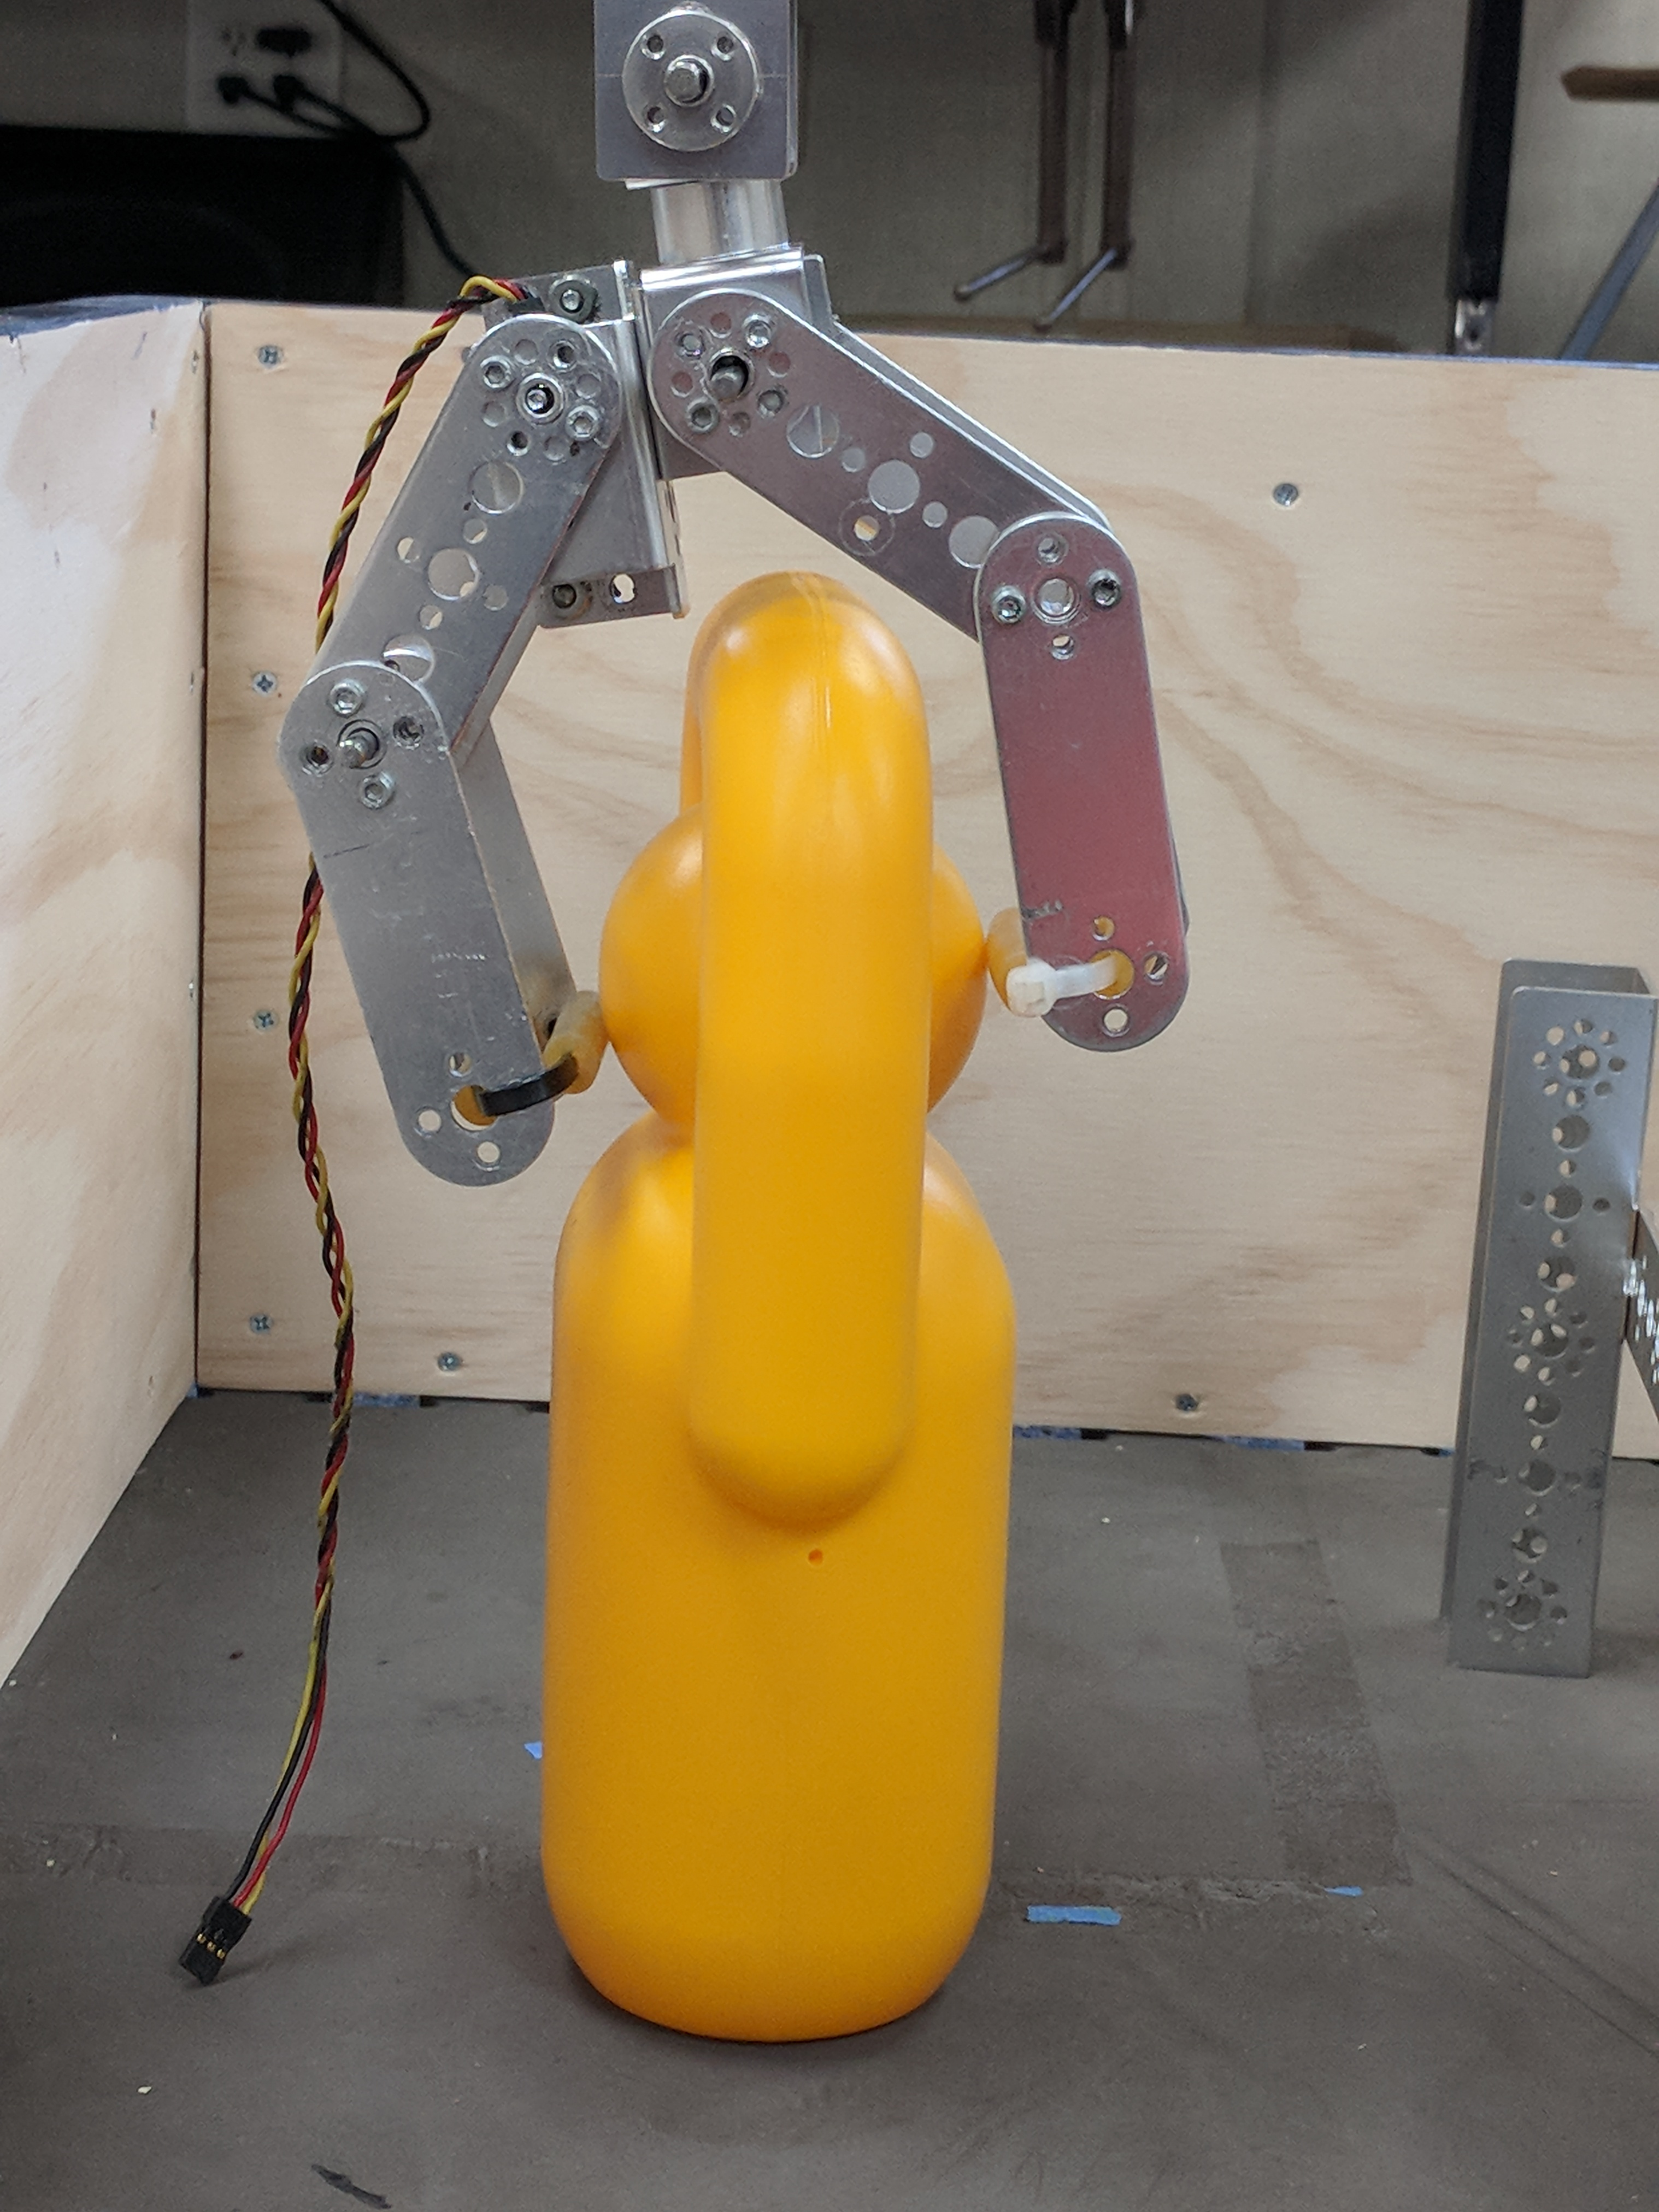
\includegraphics[width=.6\textwidth]{02/images/clawgrippingrelic.jpg}
    \caption{claw}
    \label{fig:claw}
\end{figure}

\subsection{Prepare Inventor files for the Glyph lifter}
%!Download files from GrabCAD and find files on hard drive that are necessary to create the Glyph lifter to start designing it.
John went onto GrabCAD and downloaded all parts necessary to create the Glyph lifter. John also went through the files from last year to find all useful parts for the lifter. Afterward he started the rough design of the lifter. We decided to use a lead screw for raising and lowering the mechanism because it would take up less space and be able to raise a large load. The initial design is shown in figure \ref{fig:leadscrew}. Some small changes were made from the original idea including the secondary lifting mechanism that would be necessary for the lifter to reach the fourth row, and the mounting points for the glyph holder.
\begin{figure}[h]
    \centering
    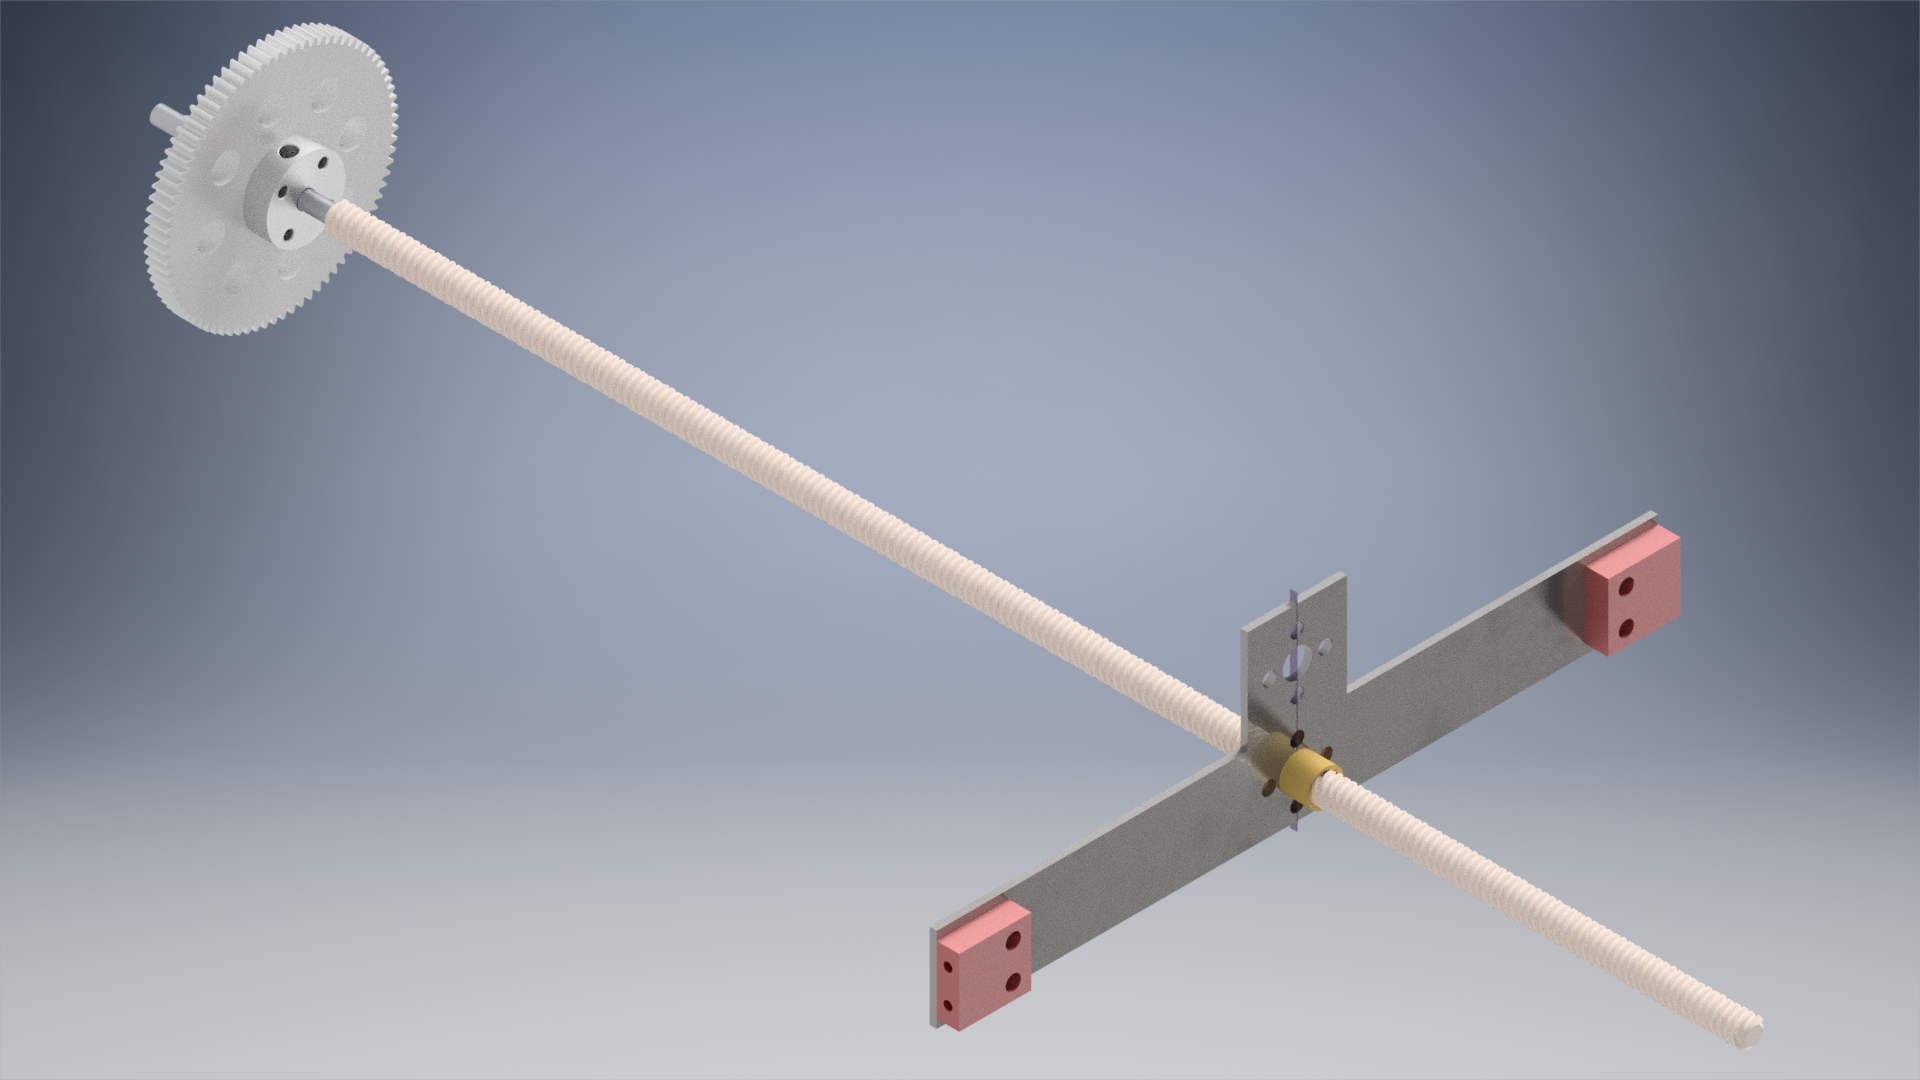
\includegraphics[width=.6\textwidth]{02/images/leadscrew.png}
    \caption{a lead screw}
    \label{fig:leadscrew}
\end{figure}

\subsection{Research the most efficient type of drivetrain}
%!Research successful drivetrains that other teams have used to win, and decide on a drivetrain to construct for this season.
Oren and Dominick did a ton of research on other teams' successful drivetrains and decided on a direction to take for the drivetrain division. They narrowed the choices down to a mecanum drive, and three variations of 6-wheeled tank drive, 6 wheel direct drive, 6 wheel with drop center, and 6 wheel with omni front and back wheels. They were able to elimane swerve drives early due to their complexity, and an omni drive because it was less reliable and provided no advantages over mecanum. The options, as well as their pros and cons, are shown in figure \ref{fig:options}. They decided that a mecanum drive would be best, because it could provide the key maneuverability necessary for aligning with the cryptobox, and there is no need for the high traction necessary in games with more defensive play. The next step for the drivetrain team is to decide how to drive each mecanum wheel.
\begin{figure}[h]
    \centering
    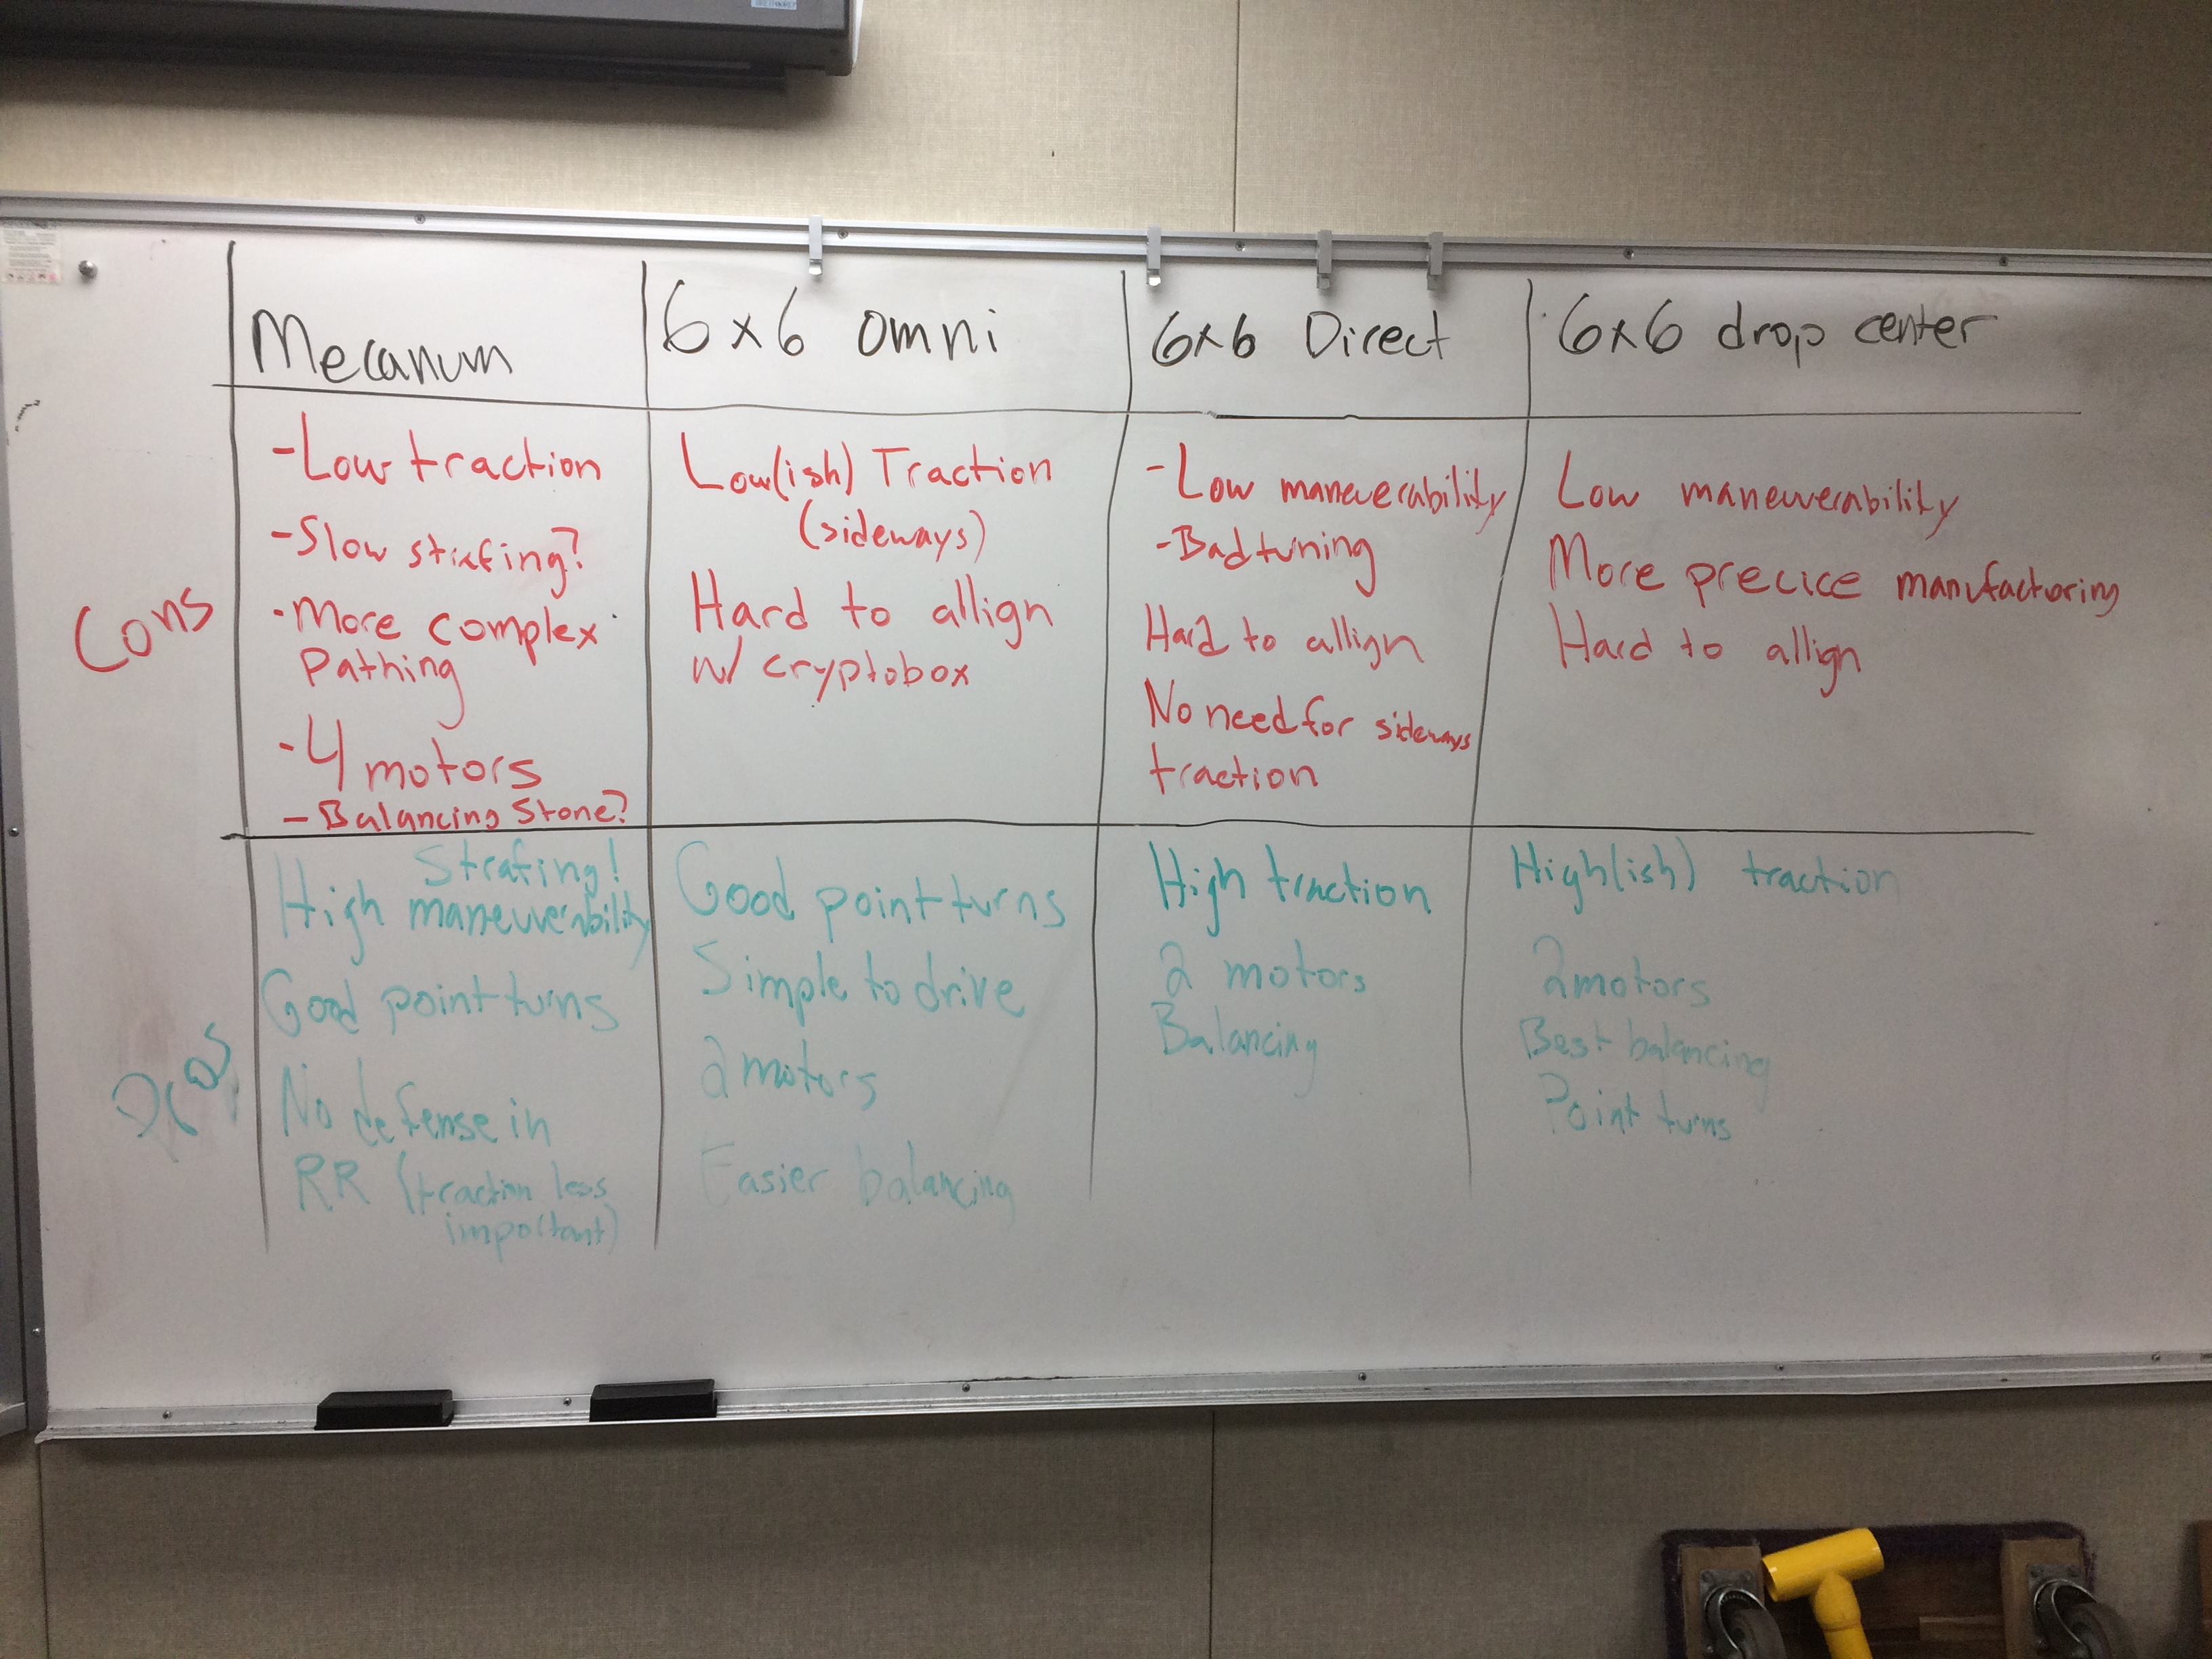
\includegraphics[width=.6\textwidth]{02/images/options.jpg}
    \caption{some of the options}
    \label{fig:options}
\end{figure}

\end{document}